\documentclass[a4paper, 10pt]{article}

\title{MOSIG M1 Visual Computing TP2}
\date{}
\author{Gilchrist N'dri \and Quoc-Trung Vuong}

\usepackage[utf8]{inputenc}
\usepackage{listings}
\usepackage{color}
\usepackage{amsmath}
\usepackage{graphicx}
\usepackage{geometry}

\geometry{a4paper, portrait, margin=1in}

\definecolor{dkgreen}{rgb}{0,0.6,0}
\definecolor{gray}{rgb}{0.5,0.5,0.5}
\definecolor{mauve}{rgb}{0.58,0,0.82}

\lstset{
  language=C,
  showstringspaces=false,
  columns=flexible,
  basicstyle={\small\ttfamily},
  numbers=none,
  numberstyle=\tiny\color{gray},
  keywordstyle=\color{blue},
  commentstyle=\color{dkgreen},
  stringstyle=\color{mauve},
  otherkeywords={gray},
  breaklines=true,
  breakatwhitespace=true,
  tabsize=2
}

\begin{document}
\maketitle
\subsection*{K-means with intensity values}
\subsubsection*{Data structure}
Each pixel is stored with the intensity values of red, green, and blue components, and x (row number) and y (column number)

\begin{lstlisting}[frame=single]
typedef struct pixel {
  unsigned char red;
  unsigned char green;
  unsigned char blue;
  unsigned int x;
  unsigned int y;
} pixel_t;
\end{lstlisting}

\subsubsection*{Algorithm}
\paragraph{Initialize cluster centers} One way to initialize cluster centers is to generate them randomly (each component can have values from 0 to maxval, i.e. 255).
\begin{lstlisting}[frame=single]
for (i = 0; i < num_clusters; i++) {
  centers[i].red = rand() % (maxval + 1);
  centers[i].green = rand() % (maxval + 1);
  centers[i].blue = rand() % (maxval + 1);
}
\end{lstlisting}

\paragraph{Determine which cluster a pixel should be in} by determining which cluster center is nearer to the pixel (which means minimum distance).
\begin{lstlisting}[frame=single]
int assign_cluster(pixel_t p, pixel_t *centers, int num_clusters) {
  float min_dist = FLT_MAX;
  int cluster_id = -1;
  for (int i = 0; i < num_clusters; i++) {
    float dist = distance(p, centers[i]);
    if (dist < min_dist) {
      min_dist = dist;
      cluster_id = i;
    }
  }
  return cluster_id;
}
\end{lstlisting}

\begin{lstlisting}[frame=single]
// Assign point to cluster
for (i = 0; i < rows * cols; i++) {
  int id= assign_cluster(pixels[i], centers, num_clusters);
  int current_size = cluster_size[id];
  clusters[id][current_size] = pixels[i];
  cluster_size[id]++;
}
\end{lstlisting}

After that, relocate each cluster center to the mean value of the respective cluster members.
\begin{lstlisting}[frame=single]
for (i = 0; i < num_clusters ; i++){
  int red = 0, green = 0, blue = 0;

  for (j = 0; j < cluster_size[i]; j++) {
    red += clusters[i][j].red;
    green += clusters[i][j].green;
    blue += clusters[i][j].blue;
  }

  red /= cluster_size[i];
  green /= cluster_size[i];
  blue /= cluster_size[i];
  centers[i] = (pixel_t) {red, green, blue};
}
\end{lstlisting}

Repeat that procedure for few cycles so that cluster centers stabilize.

\subsubsection*{Result with different initial cluster centers}
The initial cluster center choice could have major impact on the result
\begin{figure}[!htb]
\centering

\includegraphics[width=142px]{frog_rgb_3_0_out.png}
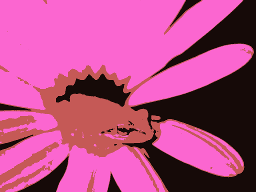
\includegraphics[width=142px]{frog_rgb_3_gray_out.png}

\includegraphics[width=142px]{frog_rgb_3_pol_out.png}
\caption[caption]{Image segmentation using k-means with 3 clusters. From left to right:\\
a. (0, 0, 0), (1, 1, 1), (2, 2, 2)\\
b. (0, 0, 0), (127, 127, 127), (127, 127, 127)\\
c. (255, 0, 0), (0, 255, 0), (0, 0, 255)}
\end{figure}

\subsubsection*{Result with different number of clusters}
The number of clusters choice could have major impact on the result
\begin{figure}[!htb]
\centering
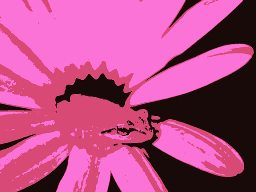
\includegraphics[width=142px]{frog_rgb_3_out.png}
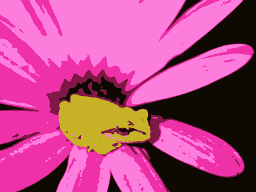
\includegraphics[width=142px]{frog_rgb_5_out.png}
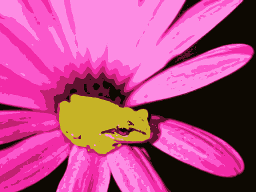
\includegraphics[width=142px]{frog_rgb_7_out.png}
\caption[caption]{Image segmentation using k-means (random initial centers). From left to right: 3, 5, 7 centers}
\end{figure}

\subsection*{Consider both intensity and location in the image}
Taking into account pixel location when computing distance could help breaking the tie for the case that k-means with just intensity values does not perform well (due to bad initialization).
\begin{figure}[!htb]
\centering
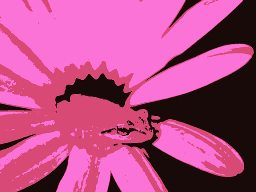
\includegraphics[width=142px]{frog_rgb_3_out.png}

\includegraphics[width=142px]{frog_rgb_loc_3_out.png}
\caption[caption]{K-means (3 clusters) with center initialized with similar intensity values (r=253, g=138, b=229). Result without and with location used for distance.}
\end{figure}

Value scale of intensity and location might differ greatly from each other. For example, if rgb components could range from 0 to 255, while the target image is large location x and y could range from 0 to 4000, then it is very likely that the location values dominate intensity values when computing and comparing distance. In order to balance the influence of intensity and location, a solution would be to normalize these values before computing the distance difference.
\end{document}
